\documentclass[9pt,twocolumn,twoside]{osajnl}


%\usepackage{csquotes}
\usepackage{tikz}
%\usepackage{graphicx}


\journal{josaa} % Choose journal (ao, josaa, josab, ol)

\setboolean{shortarticle}{false} % true = letter, false = research article


\title{On the analogy between curved space-time and non-impedance-matched anisotropic media }

\author[1]{S. A. Mousavi}
\author[2*]{R. Roknizadeh}
\author[3,4]{SH. Dehdashti}
\author[5]{S. Sahebdivan}

\affil[1]{Department of Physics, Faculty of Science, University of Isfahan, Hezar Jerib, Isfahan, 81746-73441, Iran}
\affil[2]{ Department of Physics, Quantum Optics Group, Faculty of Science, University of Isfahan, Hezar Jerib, 81746-73441 Isfahan, Iran}
\affil[3]{State Key Laboratory of Modern Optical Instrumentations, Zhejiang University, Hangzhou 310027, China}
\affil[4]{The Electromagnetic Academy at Zhejiang University, Zhejiang University, Hangzhou 310027, China}
\affil[5]{Quantum Optics, Quantum Nanophysics and Quantum Information, Faculty of Physics, University of Vienna, Boltzmanngasse 5, 1090 Wien}
\affil[*]{Corresponding author: r.roknizadeh@gmail.com}

\dates{Compiled \today}

\ociscodes{(160.1190)  Anisotropic optical materials,(160.3918) Metamaterials, (260.2110)   Electromagnetic optics }

\doi{\url{http://dx.doi.org/10.1364/ao.XX.XXXXXX}}

\begin{abstract}


An electromagnetic medium with gradient refractive index can resemble a geometrical analogy with an arbitrary curved space-time \cite{leonhardt2006general}. 
 In this paper, we show that a non-impedance-matched medium with a varying optical axis can resemble the features of an optical metric.
The medium with a varying optical axis is an engineered stratified slab of material, that in each layer, the orientation of optical axis would slightly change while the magnitude of refractive index remains constant. 
Instead of change in the refractive index, the inhomogeneity in such a medium is induced by the local anisotropy.  Therefore the propagation of light depends on the local optical axis.
We study the conditions that make the analogy between curved space-time and a medium with a varying optical axis. 
Extension of  the transformation optics to the media with optical axis profile might ease some fabrication cumbersome of  gradient refractive index materials for particular frequencies. 

\end{abstract}



\setboolean{displaycopyright}{true}

\begin{document}
\maketitle
\thispagestyle{fancy}
\ifthenelse{\boolean{shortarticle}}{\abscontent}{}

\section{Introduction}

The impedance-match condition for the medium is considered as a necessary factor that makes the geometrical analogy complete.
Therefore, this work provides an alternative means to control the light trajectory in the novel optical devices such as invisibility cloaks or analogue gravity models. 
In the last decade, the emergence of a new method to design the electromagnetic medium results in the innovative manipulation of the electromagnetic fields in optical devices \cite{pendry2006controlling}. This particular method, known as transformation optics, combines the old branches of science like geometry, physics and mathematics in a new applicable framework.
In the context of transformation optics, a properly designed electromagnetic medium, characterised by constitutive relation, can resemble a unique geometry of a particular empty space-time. The underlying principle for such a geometrical analogy is the conformal invariance of electromagnetic fields which allows a diffeomorphism between a general vacuum (called virtual space-time or electromagnetic space) and the designed medium which serves as the real space-time.  
Theoretically it was a known fact that there is an subtle relation between the light trajectories inside an inhomogeneous, anisotropic medium and the constitutive relation for the electromagnetic fields. But, just in the recent  years \cite{yao2014analogy, leonhardt2006general, thompson2011completely} the complete analysis, in term of transformation optics, reveals the essential conditions and fundamental restrictions for such an analogy in practice. 
Today, transformation optics methods is widely applied in theoretical and experimental researches such as analogue gravity \cite{bittencourt2015light, chen2010transformation,  sheng2013trapping}, invisibility cloaks \cite{mccall2013transformation, leonhardt2012geometry} and other innovative optical devices \cite{lai2009illusion, courtial2015direct, roberts2009optical, yan2008cylindrical, ma2009omnidirectional, liang2012transformation}. One of the crucial conditions  that extend the transformation optics to the full geometry framework is impedance-matched feature of the medium. An impedance-matched material is a magneto-electric medium that satisfies the condition: $\mu=\epsilon$. The term "impedance-match" refers to impedance invariant property of the medium ${\mathbf z}=\sqrt {{\epsilon}/{\mu}}=\sqrt {{\epsilon_0}/{\mu_0}}$ compare to vacuum.  An impedance-matched medium resembles some of electromagnetic responses of the vacuum.


\begin{figure}[htbp]
\centering
	 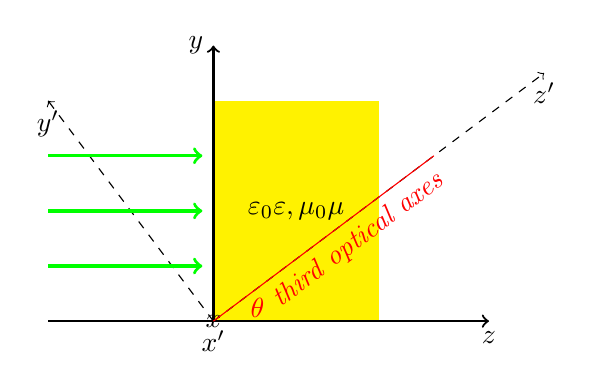
\begin{tikzpicture}[xscale=0.7, yscale=0.7]
	%-------------------- anisotropic slab --------------------------------------------------------	
	    \fill[fill=yellow] (2,0) rectangle (5,4)node [pos=0.5]{$\varepsilon_0 \boldsymbol \varepsilon, \mu_0 \boldsymbol\mu $};
	%-------------------------- coordinate--------------------------------------------
		 \draw [->,thick] (2,0) node{$x$} -- (2,5.0) node[left]{$y$} ;
		 \draw [->,thick] (-1,0) -- (7,0) node [below]{$z$};
	%------------------------- principle axes of the media ------------------------------------
		\draw [-> ,dashed] (2,0)node [below]{$x^{\prime}$} -- (8,4.5)  node [below]{$z^{\prime}$};
    \draw [-> ,dashed] (2,0) -- (-1,4) node [below]{$ y^{\prime}$};
	%---------------------------third optical axes-------------------------------------------	
	   \draw [red] (2,0) -- (6,3) node [pos=0.2, below]{$\theta$} node [pos=.6,below, rotate=37]{\textit{third optical axes}} ;		  	
	%-------------------------- light rays-------------------------------------------------------
		\draw [-> , green,very thick] (-1,1)  -- (1.8,1)  ;
	    \draw [->,green,very thick] (-1,2)  -- (1.8,2) ;
		\draw [->,green,very thick] (-1,3)  -- (1.8,3)  ;			
	\end{tikzpicture}
\caption{Schematic of an anisotropic slab with $\boldsymbol{\varepsilon}$ and $\boldsymbol{\mu}$ as a tensor, light incidents from left and incident plane is $y-z$ plane; two principle axes of media  $z^{\prime}$ and $y^{\prime}$ do not lay on the $z$ and $y$ coordinate.}
	\label{figure1}
\end{figure}

Unfortunately, such impedance-matched materials, aside from the vacuum, have been rarely found in nature; thus, it needs to design and build them artificially. 
Growing development in the metamaterial technologies \cite{cai2010optical}, brings the hope that vast range of artificial media with unusual electric and magnetic property eventually can be accomplished in practice. 
However, fabrication of artificial materials is yet in its infancy. Therefore, a realization of complex artificial materials like an impedance-matched medium in the broadband of frequencies is not a trivial task. 
Apparently, it would be of a great advantage if there were an alternative way to avoid the technically cumbersome fabrication \cite{narimanov2009optical, lee2014elliptic, dehdashti2013analogue, visser2013survey, robertson2012theory, wang2011cylindrical, bai2010controllable} and related expenses.
In the scientific literature, people ease the impedance-match condition by using the polarized light and the planar medium which scarifying some components of the light. \cite{leonhardt2012geometry}. This approach would restrict the control of light to one single polarization. Therefore, the optical device naturally has not the full functionality. 
 In such a setup, for the TE mode, electrical components of the field, a simple planar medium with electrical anisotropy can appears as an effective 2-dimensional geometry. The TM mode, or as it called in-plane polarization is totally omitted thus, cannot experience any geometry \cite{leonhardt2012geometry, sahar}. 
 Another example to avoid the problem is to use the coordinate rescaling to force the purely electrical medium act as a magneto-electric material in the ranges larger than wavelength\cite{danner2011controlling}. 


Anisotropy and inhomogeneity in the medium is responsible for curving the light trajectories. In medium with a varying optical axis inhomogeneity is due to infinitesimal change of optical axis in each layer. 
We know that in the anisotropic materials the propagation of light depends on the direction of optical axis, therefore, it is convenient to start  studying the propagation of light in a birefringent layer and introducing the methods to derive the infinitesimal optical length.
Inspired by the ray tracing methods, we derive the conformal metric for the normal incident on the slab of anisotropic birefringent material when the propagation of light is depend on the axis.
 As a result we show there is an independent metric associated to each polarization of the light field in a birefringent medium.

Birefringent media are quite common in nature and also much cheaper to design artificially. Crystals are the best-known materials that perform electrical anisotropy based on their particular crystal structure and the symmetry of their space group. Many plastics also are birefringent, because their molecules are 'frozen' in a stretched conformation when the plastic is molded or extruded \cite{PEN}. 
 
The advantage of our method compared to planar media is that , in principle, the optical manipulation would not be limited to TE mode, but both polarization have their own optical metric. Considering this property, there is a opportunity to explore the study of optical devices with double functionality \cite{}.
 
 Finally, as another alternative to impedance-match condition, we investigate the optical properties of a medium with a variable optical axes. Using the ray-tracing method, we obtain the trajectory of light  for two arbitrary axes orientation. We conclude that a medium with the variable optical axes can consider as a curved space for light rays. They show the capacity for being used in transformation optics designs when impedance-matched materials are costly. More elaborated theory of transformation optics with variable optical axes profile would appear shortly in the further publications.

The organization of the paper is as follows: In section 2 we briefly describe our material and methods used in this research. In section 3, we explain a technique, eigenvalue wave equation method,  to solve the Maxwell equations in a general inhomogeneous anisotropic medium when the geometrical optics limit is hold. In this section, we derive the path elements of light propagation in an anisotropic inhomogeneous medium. 
In section 4, above method is applied to a purely electric and an impedance-matched anisotropic slab respectively. 
In section 5, the optical path line elements for light in purely electric media and impedance-matched media and their corresponding metrics are compared. The idea of the medium with variable optical axes is introduced. 
Finally in section 6, some results and remarks are summarized. 

\section{Birefringent material as an alternative to impedance-matched media; Method}

A birefringent medium is an anisotropic material. \footnote{In this paper, by anisotropy we mean electrical anisotropy. However, magnetic anisotropy and, therefore, magnetic birefringence is possible. But, in most of the natural materials, at optical frequencies, the value of magnetic permeability does not significantly deviate from vacuum's magnetic permeability. Therefore, induced magnetic birefringence is not practical.}
In these anisotropic materials, the light ray divides into the ordinary and extraordinary parts. This feature is called birefringence \cite{saleh1991fundamentals, born1999principles, yariv1984optical}. 
For most of birefringent media there are two different refractive indexes associated with two normal modes. The incident light waves split into these ordinary and extraordinary modes, base on their polarization and angle of incident. 


We will show that a birefringent medium with a  refractive index profile $n^2_i= \epsilon_i , \; i=1,2$  induces different optical metrics for each TM and EM polarizations.  
For that, we need to compare the field elements for light propagation in both media. Our mathematical method to derive the light path elements is based on the eigenvalue wave equation. We calculate the optical line element in each media: first a slab of a purely electric birefringent medium that can be inhomogeneous in principle (we call it Electrical Medium) and second an impedance-matched medium that we assume that it is anisotropic in general. 
Accordingly we can construct the effective space-time metrics for each medium.
We show that the optical line element in the impedance-matched medium is equal to the optical line element for the extraordinary path in the pure electric medium therefore both induce the same optical metric.
The optical metric for the extraordinary mode in birefringent medium is associated to  the impedance-matched counterpart with $n^2= \epsilon \mu$ while $n^2=n^2_1$. 


In the impedance-matched medium, the incident light would not split. Then, the propagation direction would be identical to the extraordinary light direction in the birefringent slab. 
One can conclude that the electric birefringent medium appears for TM polarized light as good as the impedance-matched medium for non-polarized light.  By good we mean, conditions that make the geometry exact. We can consider this important result as an extension of transformation optics to non-impedance-matched media.
 As an example, we derive the profile of a birefringent electric medium in which ordinary modes feels the Rindler metric.

In the birefringent medium,  only the optical metric of extraordinary mode depends on two parameters; the principle values of the permittivity tensor and orientation of the optical axes. By changing the the orientation of optical axes for the extraordinary mode one can control and manipulate the propagation of extraordinary polarization inside the medium. This method might be a new development into a easier and cheaper manipulation of electromagnetic fields.


\section{Maxwell equations in the inhomogeneous anisotropic media}\label{Maxwell's equations in the homogeneous anisotropic media}

An inhomogeneous anisotropic material is the most general form of the electromagnetic medium. Solutions of Maxwell equations in general is not always analytically achievable in an arbitrary inhomogeneous medium. But, under some conditions and approximations we can find solutions. 
The electric and magnetic response of such a medium is fully described by the tensorial character of permittivity and permeability matrices.
 Inhomogeneity in the refractive index is result of position dependency of matrix elements of either  $\boldsymbol{\varepsilon}$ or $\boldsymbol{\mu}$  tensors. 
 
 Maxwell's equations in an inhomogeneous anisotropic source-free materials, $\rho=0, \quad \mathbf{J}=0 $,  are given by \cite{jackson1962classical}:

\begin{gather}
\nabla\cdot \mathbf{D} =0,\quad \nabla\cdot \mathbf{B} =0, \nonumber \\
\nabla\times\mathbf{E}=-\dfrac{\partial\mathbf{B}}{\partial t}, \quad \nabla\times\mathbf{H} =\dfrac{\partial\mathbf{D}}{\partial t}.\label{m.h}
\end{gather}
While the constitutive relations are hold as:
 \begin{equation} 
 \mathbf {D}=\varepsilon_0 \boldsymbol \varepsilon \mathbf{E},  \qquad
  \mathbf{B}=\mu_0 \boldsymbol\mu \mathbf{H},
  \end{equation}
where $\boldsymbol{\varepsilon}$ and $\boldsymbol{\mu}$  are respectively the electric permittivity and  the magnetic permeability tensors for an arbitrary optical axis. 

 Explicitly assuming anisotropy and  inhomogeneity , wave equation can be written as
\begin{equation}
\mathbf{\nabla}\times{\boldsymbol{\mu^{-1}}(\mathbf{\nabla}\times\mathbf{E})}=-\mu_{0}\dfrac{\partial^{2}}{{\partial{t}}^{2}}\mathbf{D}.
\label{eq3}
\end{equation}

In a homogeneous anisotropic medium, the plane waves, $ \mathbf{E}\propto \exp\left[i\mathbf{k} \cdot  \mathbf{r}- i\omega t \right]$, is usually assumed as the general solution of the Maxwell wave equation \cite{hao2008electromagnetic}. Therefore, Eq. (\ref{eq3}) becomes:
   
   %------------------------------------------------------------------------------------------------------------
   \begin{equation}\label{w.eq}
	\mathbf{k}\times{\boldsymbol{\mu^{-1}}(\mathbf{k}\times\mathbf{E})}=-k^{2}_{0}\boldsymbol{\varepsilon}\mathbf{E}.
\end{equation}

While, in the inhomogeneous anisotropic media the wave vector is a function of position. Under particular conditions, $\lambda\rightarrow 0$, quasi plane waves (Appendix A) , as described below, can be used as general solutions of the Maxwell equations in a inhomogeneous  medium \cite{born1999principles, sluijter2010ray}, 

\begin{equation} 
\{\mathbf{E,H}\}(\mathbf{r},t)=\{\mathbf{E,H}\}(\mathbf{r})e^{-i\varphi(\mathbf{r},t)}
\label{form}
\end{equation}
 Where, the wave vector $\mathbf{k}$ and the angular frequency $\omega$ of this quasi plane wave are defined as 
\begin{equation}\label{wave}
\mathbf{k}=\nabla{\varphi(r,t)}=k_{0}\nabla{\psi}, \qquad
\omega=-\dfrac{\partial{\varphi(r,t)}}{\partial{t}}.
\end{equation}
If  the wave has a constant angular frequency, $\omega=constant$, we can write the phase term of the (\ref{form}) as 
\begin{equation}
\varphi(\mathbf{r},t)=k_{0}\psi(\mathbf{r})-\omega t ,
\end{equation}
where $k_{0}$  is the wave number in vacuum and $\psi(\mathbf{r})$ is the function of the optical path.

Using quasi plane wave, (\ref{form}), the Maxwell's equations in inhomogeneous anisotropic media can be written as, 
\begin{gather}
\boldsymbol{\nabla}{\psi}\cdot\mathbf{D}=-\dfrac{1}{ik_{0}}\boldsymbol{\nabla}\cdot \mathbf{D}, \nonumber\\
\boldsymbol{\nabla}{\psi}\cdot \mathbf{B}=-\dfrac{1}{ik_{0}}\boldsymbol{\nabla}\cdot \mathbf{B},\nonumber\\
\boldsymbol{\nabla}{\psi}\times\mathbf{E}-c\mathbf{B}=-\dfrac{1}{ik_{0}} \boldsymbol{\nabla}\times\mathbf{E},\nonumber\\
\boldsymbol{\nabla}{\psi}\times\mathbf{H}+c\mathbf{D}=-\dfrac{1}{ik_{0}} \boldsymbol{\nabla}\times\mathbf{H},\label{m.i}
\end{gather}
where $c={1}/{\sqrt{\mu_{0}\varepsilon_{0}}}$.

In geometrical optics regime, we assume $k_{0}\gg1$ and $\boldsymbol{\nabla}\cdot \mathbf{D}/k_{0}\ll 1$. So the right hand  sides of the above equations (\ref{m.i}) can be neglected  and these equations become similar to (\ref{m.h}), the Maxwell equations in homogeneous anisotropic media. Therefore, the wave equation in inhomogeneous anisotropic media can be obtained as, 

\begin{eqnarray}
\boldsymbol{\nabla}{\psi}\times{\boldsymbol{\mu^{-1}}(\boldsymbol{\nabla}{\psi}\times\mathbf{E})}=-\boldsymbol{\varepsilon}\mathbf{E}.
\end{eqnarray}
Multiplying above equation by $k_{0}$, the wave equation in inhomogeneous anisotropic media take the following form, which is equivalent with the relation(\ref{w.eq}).

\begin{eqnarray}\label{wave equations}
\mathbf{k} \times{\boldsymbol{\xi}(\mathbf{k}\times\mathbf{E})}=-k^{2}_{0}\boldsymbol{\varepsilon}\mathbf{E},
\end{eqnarray}
where we defined $\boldsymbol{\xi}=\boldsymbol{\mu}^{-1}$.

We rewrite the equation (\ref{wave equations}) in a matrix equation form, 
\[\mathbf{M}\mathbf{E}=-k_{0}^{2}\boldsymbol{\varepsilon}\mathbf{E}, \] 
in which  the matrix elements of $\mathbf{M}$ are obtained as

\begin{align}
M_{11}&=2\xi_{23}k_{z}k_{y}-(\xi_{33}k_{y}^{2}+\xi_{22}k_{z}^{2}), \nonumber\\
M_{12}&=\xi_{21}k_{z}^{2}-\xi_{23}k_{z}k_{x}-\xi_{31}k_{z}k_{y}+\xi_{33}k_{y}k_{x}, \nonumber\\
M_{13}&=\xi_{31}k_{y}^{2}-\xi_{23}k_{y}k_{x}-\xi_{21}k_{z}k_{y}+\xi_{22}k_{z}k_{x}, \nonumber\\
M_{22}&=2\xi_{13}k_{z}k_{x}-(\xi_{33}k_{x}^{2}+\xi_{11}k_{z}^{2}), \nonumber\\
M_{23}&=\xi_{32}k_{x}^{2}-\xi_{12}k_{z}k_{x}-\xi_{31}k_{y}k_{x}+\xi_{11}k_{y}k_{z},\nonumber\\
M_{33}&=2\xi_{21}k_{x}k_{y}-(\xi_{22}k_{x}^{2}+\xi_{11}k_{y}^{2}).
\end{align}


\subsection{Eigenvalue equation; method}
In an inhomogeneous anisotropic material, the direction of the electric and magnetic fields, $\mathbf{E}$ and $ \mathbf{H}$,  can vary inside the medium. However, the direction of the displacement, $\mathbf{D}$, and induction field, $\mathbf{B}$, are constant. \textcolor{blue}{In an inhomogeneous anisotropic material for a known wave vector the directions of the displacement, $\mathbf{D}$, and induction field, $\mathbf{B}$, through the equations $\nabla\cdot \mathbf{D} =0 $ and $\nabla\cdot \mathbf{B} =0$, are clear but  the directions of the electric and magnetic fields, $\mathbf{E}$ and $ \mathbf{H}$,  can vary inside the medium.} Therefore, it is useful to write the wave equation in the form of eigenvalue equation for $\mathbf{D}$  \cite{saleh1991fundamentals}. 
By substituting $\boldsymbol{\nabla}{\psi}=n\hat{U}$ in Eq. (\ref{w.eq}), we get eigenvalue equation, 

\begin{equation}\label{d.w.eq}
    \hat{U}\times{\boldsymbol{\xi}(\hat{U}\times\boldsymbol{\eta}\mathbf{D})}=-\frac{1}{n^{2}}\mathbf{D},
\end{equation}
where  $\boldsymbol{\eta}=\boldsymbol{\varepsilon}^{-1}$. For each direction of the wave vector we find  two directions for $\mathbf{D}$.\\
 The Eq. (\ref{d.w.eq}) can be written in operator form,

\begin{equation}\label{m.f}
\mathbf{L}\mathbf{D}=-\frac{1}{n^{2}}\mathbf{D}.        
\end{equation}
In a general coordinate, matrix  $L$ might has a complicated form. Nevertheless, knowing that the light propagates in a plane, we can establish a fixed coordinate system such that the propagation plane coincides with one of the principal planes of the coordinate system. As  Fig. \ref{figure1} shows, we choose the $y-z$ as the propagation plane, so the $x$ component of  the wave vector vanishes.  Thus,  matrix $L$ simplifies to the following non-zero components:

\begin{align}
L_{1i} &= (\xi_{31}\eta_{3i}-\xi_{33}\eta_{1i})u^{2}_{2} +(-\xi_{22}\eta_{1i}+\xi_{21}\eta_{2i})u^{2}_{3}\nonumber\\
&\qquad +(2\xi_{23}\eta_{1i}-\xi_{31}\eta_{2i}-\xi_{21}\eta_{3i})u_{2}u_{3},\nonumber\\
L_{2i} &=(\xi_{12}\eta_{1i}-\xi_{11}\eta_{2i})u^{2}_{3}+(-\xi_{13}\eta_{1i}+\xi_{11}\eta_{3i})u_{2}u_{3}, \nonumber \\
L_{3i} &=(\xi_{13}\eta_{1i}-\xi_{11}\eta_{3i})u^{2}_{2}+(-\xi_{12}\eta_{1i}+\xi_{11}\eta_{2i})u_{2}u_{3},
 \end{align}
where $i=1,2,3$.

One can obtain Electrical displacement $\mathbf{D}$  by solving  Eq. (\ref{m.f}) through matrix algebra:


\begin{equation}\label{det}
    \det(\mathbf{L}+\frac{1}{n^{2}}\mathbf{I})=0,
\end{equation}

Having the components of  $\mathbf{D}$, other fields and the Poynting vector can be calculated easily  \cite{jackson1962classical}

\begin{equation}\label{e.h}
\mathbf{E}=\frac{\boldsymbol\eta}{\varepsilon_{0}}\mathbf{D}, \hspace{.5cm}  \mathbf{B}=n\sqrt{\mu_{0}\varepsilon_{0}}  \hat{U}\times{\mathbf{E}}, \hspace{.5cm}\mathbf{H}=\frac{\boldsymbol\xi}{\mu_{0}}\mathbf{B},
\hspace{.5cm}\mathbf{S}=  \mathbf{E}\times \mathbf{H}.
\end{equation}

Finally, the direction of the field propagation for each mode is determined from the Poynting vector as: 

\begin{equation}\label{p.v}
\dfrac{\mathbf{\mathrm{d}{r}}}{\mathrm{d}{l}}=\dfrac{\mathbf{S}}{S}.
\end{equation}

\subsection{Riemannian metric for the medium} \label{rim}

To derive the Riemannian metric we need to have the optical line element in the propagation medium.
The surface of equal phases for the propagating light fields define as the solutions of:

\begin{equation}\label{level}
\mathrm{d}{\varphi(r,t)}=0.
\end{equation}

Adopting the definitions from  Eqs. (\ref{form}) and (\ref{wave}), we can rewrite the Eq. (\ref{level}) for the wave fronts as:

\begin{equation}\label{phase1}
\mathbf{\nabla}{\varphi(r,t)}\cdot \mathbf{\mathrm{d}{r}}-\omega\mathrm{d}{t}=0.
\end{equation}

During the time interval  $\mathrm{d}{t}$,  the optical length in an arbitrary vacuum is given by

\begin{equation}\label{length}
\mathrm{d}{r_{v}}=\boldsymbol{\nabla}{\psi(\mathbf{r})}\cdot \mathbf{\mathrm{d}{r}},
\end{equation}

 where index $v$ stands for vacuum.  Therefore, we can write the line element in space-time as 

\begin{equation}
\mathrm{d}s^{2}=-c^{2}\mathrm{d}{t}^{2}+{\mathrm{d}}{r^{2}_{v}}.
\end{equation}

Therefore the Eq. (\ref{length}) becomes:

\begin{equation}\label{a}
{\mathrm{d}}{r^{2}_{v}}={\mathrm{d}{\mathbf{r}}}^{T}\left(\boldsymbol{\nabla}{\psi(\mathbf{r})}\otimes\boldsymbol{\nabla}{\psi(\mathbf{r})}\right)\mathbf{\mathrm{d}{r}}.
\end{equation}

Such that, the optical path length (OPL) takes the following form

\begin{equation}
OPL\equiv\int{\sqrt{{\mathrm{d}}{r^{2}_{v}}}}=\int{\sqrt{{\mathrm{d}{\mathbf{r}}}^{T}\mathbf{n}_{p}^{2}\mathbf{\mathrm{d}{r}}}},
\end{equation}
in which, 
\begin{equation}\label{fr}
\mathbf{n}_{p}^{2}=\boldsymbol{\nabla}{\psi(\mathbf{r})}\otimes\boldsymbol{\nabla}{\psi(\mathbf{r})}.
\end{equation}

In Eq. (\ref{fr}), the $\mathbf{n}_{p}^{2}$ denotes the square of the phase refractive index, which appears as a tensor.  According to relations (\ref{wave}) and (\ref{length}),  $\boldsymbol{\nabla}{\psi(\mathbf{r})}$ is the gradient of the phase refractive vector, $\mathbf{n}_{p}=\boldsymbol{\nabla}{\psi(\mathbf{r})}=\mathbf{k}/k_0$ which is normal to the wave front. So we can write $\mathbf{k}=k_{0}\boldsymbol{\nabla}{\psi(\mathbf{r})}=k_{0}n_{p}\hat{U}$. Therefore, in eigenvalue wave equation (\ref{d.w.eq}),  $n$ also must refer to the phase refractive index \cite{born1999principles}.\\


In anisotropic media the ray direction is not necessarily along the wave vector, so it is appropriate to define the ray refractive index, $n_{ray}$. Ray refractive index defines as the ratio between optical line element, $dr_{v}$ and the line element in medium, dr, \cite{born1999principles}

\begin{equation}\label{ray-refractive}
n^{2}_{ray}=\dfrac{{\mathrm{d}{r^{2}_{v}}}}{{\mathrm{d}{l}^{2}}}.
\end{equation} 
Using relation (\ref{a}), we can write ray refractive index as 
\begin{equation}\label{r.refractive}
n^{2}_{ray}={\dfrac{\mathrm{d}{\mathbf{r}}}{\mathrm{d}{l}}}^{T}\left(\boldsymbol{\nabla}{\psi(\mathbf{r})}\otimes\boldsymbol{\nabla}{\psi(\mathbf{r})}\right)\dfrac{\mathrm{d}{\mathbf{r}}}{\mathrm{d}{l}}.
\end{equation}
Hence, we can write space-time line element in term of phase refractive index or equivalently in term of ray refractive index,

\begin{align}
\mathrm{d}s^{2}=-c^{2}\mathrm{d}{t}^{2}+{\mathrm{d}{\mathbf{r}}}^{T}\mathbf{n}^{2}_{p}\mathbf{\mathrm{d}{r}},\label{p.element}
\end{align}
\begin{align}
\mathrm{d}s^{2}=-c^{2}\mathrm{d}{t}^{2}+n^{2}_{ray}\mathrm{d}{l}^{2}.
\label{r.element}
\end{align}

The ray trajectory specifies the geodesic of the effective geometry.  But in anisotropic materials, ray trajectory might differ from the direction of the wave vector.  Thus, to determining the effective geometry we need to take the optical line element (\ref{r.element}) expressed in terms of the ray refractive index.
 The optical line element (\ref{r.element}), specifies the effective metric component in accordance  with the line element of the Riemann geometry (\ref{line element}), 
 
\begin{equation}\label{line element}
\mathrm{d}s^{2}=g_{\mu\nu}dx^{\mu}dx^{\nu},
\end{equation}

where $ g_{\mu\nu} $ is the metric tensor. 

However,  in the isotropic media  or any case that the direction of the rays is along the wave vector the line element (\ref{p.element}) can be used in determine the effective geometry.

\textcolor{blue}{ The ray trajectory specifies the geodesic of the effective geometry.  But in anisotropic materials, ray trajectory might differ from the direction of the wave vector.  Thus, to determining the effective geometry we need to take the optical line element (\ref{r.element}) expressed in terms of the ray refractive index. However,  in the isotropic media  or any case that the direction of the rays is along the wave vector the line element (\ref{p.element}) can be used in determine the effective geometry. The optical line element (\ref{r.element}), specifies the effective metric component in accordance  with the line element of the Riemann geometry (\ref{line element}), }
 
\begin{equation}\label{line element}
\mathrm{d}s^{2}=g_{\mu\nu}dx^{\mu}dx^{\nu},
\end{equation}

where $ g_{\mu\nu} $ is the metric tensor. \textcolor{blue}{A glance at the above relations (\ref{r.element}) and (\ref{line element}) results the conformally flat spaces for the spatial term of the effective geometry.  In fact, the line element (\ref{r.element}) specifies propagation plane as an conformally flat spaces. }

\section{Normal incident of light on a piece of electromagnetic slab} \label{general-normal}

In this section, we investigate the behavior of the perpendicular incident light on an anisotropic slab of material.
Our analyse is easily extendable to an arbitrary angle of incidence.
It is well known that in the normal incidence, the direction of the wave vector does not change.  We assume $y-z$ plane as the propagation plane, while, the light comes parallel to the $z$ axis. Therefore:  

\begin{eqnarray}\label{pt}
|\mathbf{k}|=k_{z} \quad\rightarrow \quad {n}^{2}_{p}=n^{2}_{zz}.
\end{eqnarray} 

Further, we assume that  two principal axes  $y^{\prime}$ and $z^{\prime}$ of the slab lay in this $y-z$ plane, Fig. \ref{figure1}.
In this case the dielectric tensor can be obtained from following relation \cite{yeh1980optics},

 \begin{eqnarray}\label{t.t}
		\boldsymbol{\varepsilon}= \mathbf{A} \boldsymbol{\varepsilon^{\prime}}\mathbf{A}^{T},
\end{eqnarray}
where $ \boldsymbol{\varepsilon^{\prime}} = \mbox{diag} (\varepsilon_{1},\varepsilon_{2},\varepsilon_{3})$ are  principle permittivity tensors and $\mathbf{A}$  is the rotation matrix, which describes the rotation of the coordinate axes with respect to the crystal principle axes and $ \mathbf{A}^{T}$ is transpose of the rotation matrix $ \mathbf{A}$.

Suppose that two principal axes  $y^{\prime}$ and $z^{\prime}$ of the slab lay in this plane, Fig. \ref{figure1}, then the rotation matrix is given by
 
\begin{align}\label{r.m}
        \mathbf{A}=\mathbf{R}_{x}(\theta)=
        \begin{pmatrix}
            1&0&0 \\
            0&\cos{\theta} &\sin{\theta} \\
            0&-\sin{\theta} & \cos{\theta}
        \end{pmatrix},
\end{align}
where $\theta$ is a angle between $z$ and $z^{\prime}$.  From Eq. (\ref{t.t}),  we can obtain the rotated permittivity tensor,

\begin{align}\label{eps}
        \boldsymbol{\varepsilon}=
        \begin{pmatrix}
             \varepsilon_{1} &0 &0 \\
            0&\varepsilon_{2} \cos^{2}{\theta} + \varepsilon_{3}\sin^{2}{\theta}   &-(\varepsilon_{2}-\varepsilon_{3})\sin{\theta}\cos{\theta} \\
            0&-(\varepsilon_{2}-\varepsilon_{3})\sin{\theta}\cos{\theta} &\varepsilon_{2} \sin^{2}{\theta} + \varepsilon_{3}\cos^{2}{\theta}
        \end{pmatrix}.
\end{align}
and also the inverse permittivity tensor,

\begin{align}\label{eta}
        \boldsymbol{\eta}= \frac{1}{\varepsilon_{2} \varepsilon_{3}}
        \begin{pmatrix}
            \frac{\varepsilon_{2} \varepsilon_{3}}{\varepsilon_{1}}& 0  &0 \\
            0&\varepsilon_{2} \sin^{2}{\theta} + \varepsilon_{3}\cos^{2}{\theta}   & (\varepsilon_{2}-\varepsilon_{3})\sin{ \theta} \cos {\theta} \\
            0& (\varepsilon_{2}-\varepsilon_{3})\sin{\theta}\cos{\theta} &\varepsilon_{2} \cos^{2}{\theta} + \varepsilon_{3}\sin^{2}{\theta}
        \end{pmatrix}.
\end{align}

From Maxwell equations we have $\boldsymbol{\nabla}\cdot \mathbf{D}=0$, hence, for  the normal incident it reads as ${D}_{z}=0$.  
For other components of the $\mathbf{D}$ by replacing relation (\ref{eta}) in (\ref{d.w.eq}), we would have:

\begin{eqnarray}\label{z.d.eq}
        \begin{pmatrix}
            - \eta_{11} \xi_{22}  & \xi_{21}\eta_{22} \\
             \eta_{11} \xi_{12}& -\xi_{11}\eta_{22}
        \end{pmatrix}
        \begin{pmatrix}
            D_{x} \\ D_{y}
        \end{pmatrix}
        = -\frac{1}{n^{2}}
        \begin{pmatrix}
            D_{x} \\ D_{y}
        \end{pmatrix}.
        %\end{align}
\end{eqnarray}
Applying the condition (\ref{det}), the eigenvalues of the Eq. (\ref{z.d.eq}) are obtained from the following equation:

\begin{equation}\label{gn}
 \left( \dfrac{1}{n^2}- \eta_{11} \xi_{22}\right)\left(\dfrac{1}{n^2}-\xi_{11}\eta_{22}\right)-\xi_{21}^{2}\eta_{22}\eta_{11}=0
\end{equation}

This is a quadratic equation in terms of $1/n^2$ which has two eigenvalues;

\begin{equation}\label{general-n}
\dfrac{1}{n^2}=\dfrac{1}{2} \left( \eta_{11} \xi_{22}+\xi_{11}\eta_{22}\right)\pm \sqrt{\left(\eta_{11} \xi_{22}-\xi_{11}\eta_{22}\right)^{2}+4\xi_{21}^{2}\eta_{11}\eta_{22}}.
\end{equation}
Corresponding eigenvectors would determine the physical components of the field. 

In the rest of this section, we investigate two special examples: the electric slab, with $\boldsymbol \mu=1$, and the impedance-matched slab, with $\boldsymbol \mu = \boldsymbol \varepsilon $. 

\subsection{Birefringent medium}\label{electric anisotropic}

For the purely electric medium, the refractive indices (\ref{general-n}) are given by

\begin{eqnarray}
        &n_{o}^2=\varepsilon_{1} \label{n1},\\
        &n^{2}(\theta)=\dfrac{\varepsilon_{2}\varepsilon_{3}}{\varepsilon_{2}\sin^{2}{\theta}+\varepsilon_{3}\cos^{2}{\theta}} \label{n2}.
\end{eqnarray}    

Relation (\ref{n2}) shows the refractive index depends on principle values of the permittivity tensor, i.e, $\varepsilon_{2}$ and $\varepsilon_{3}$, and, $\theta$, the angle between  the direction of the wave vector and third principle axis. Whereas the refractive index (\ref{n1}) only depends on $\varepsilon_{1}$.

For a specific angle of incident, in this example perpendicular incident, there is two modes associated to the above refractive indices profiles. 

For refractive index (\ref{n1}), we obtain $\mathbf{D}$ by solving the eigenvalue equation (\ref{z.d.eq}):

\begin{align} \label{mod-n1}
        \mathbf{D}=D_{x}
         \begin{pmatrix}
            1 &0&0
         \end{pmatrix}^{T}.    
\end{align}

and for the refractive index (\ref{n2}) we have:

 \begin{eqnarray}\label{mod-n2}
  \mathbf{D}=D_{y}
\begin{pmatrix}
0&1&0
\end{pmatrix}^{T}.
 \end{eqnarray}
 
By applying the normalization condition, $\mathbf{E}\cdot \mathbf{E}=1$, we can determine the components $D_{x} $ and $D_{y} $. 
For the first normal mode (\ref{mod-n1}), electric and magnetic fields are written in the from (\ref{e.h}),

\begin{align}\label{field-n1}
\mathbf{E}=
         \begin{pmatrix}
             1\\0\\0
         \end{pmatrix},
        \qquad
         \mathbf{H}=\left(\frac{\varepsilon_{0}}{\mu_{0}}\right)^{\frac{1}{2}}(\varepsilon_{1})^{\frac{1}{2}}
         \begin{pmatrix}
            0\\1\\0
        \end{pmatrix}.
\end{align}

We can see that the normal mode is TE polarized light. Electrical component is lies in the propagating plane $y-z$.
 For second normal mode (\ref{mod-n2}),  $\mathbf{E}$ and $\mathbf{H}$ are given by,

 \begin{eqnarray}
\mathbf{E}=\left(\varepsilon_{2}^{2} \sin^{2}{\theta} + \varepsilon_{3}^{2}\cos^{2}{\theta}\right)^{-\frac{1}{2}}
 \begin{pmatrix}
 0\\ \varepsilon_{2} \sin^{2}{\theta} + \varepsilon_{3}\cos^{2}{\theta}\\ (\varepsilon_{2}-\varepsilon_{3})\sin{\theta}\cos{\theta}
 \end{pmatrix},
\end{eqnarray}
\begin{eqnarray}
 \mathbf{H}=\left(\frac{\varepsilon_{0}}{\mu_{0}}\right)^{\frac{1}{2}}\left(\dfrac{\varepsilon_{2}\varepsilon_{3}\left(\varepsilon_{2} \sin^{2}{\theta} + \varepsilon_{3}\cos^{2}{\theta}\right)}{\varepsilon_{2}^{2}\sin^{2}{\theta}+\varepsilon_{3}^{2}\cos^{2}{\theta}}\right)^{\frac{1}{2}}
 \begin{pmatrix}
 -1\\0\\0
 \end{pmatrix}.
 \end{eqnarray}
It is worth mentioning that, while the TE polarized field is propagating along the electric flux density, modes with TM polarization do not. The Poynting vectors of TE and TM polarizations can derive as

 \begin{equation}\label{ordinary-s}
\mathbf{S}_{TE}= \left(\frac{\varepsilon_{0}}{\mu_{0}}\right)^{\frac{1}{2}}(\varepsilon_{1})^{\frac{1}{2}}
 \begin{pmatrix}
 0\\0\\1
 \end{pmatrix},
  \end{equation}
 
  \begin{align}\label{extra.s}
 \mathbf{S}_{TM}= \left(\frac{\varepsilon_{0}}{\mu_{0}}\right)^{\frac{1}{2}} &\dfrac{(\varepsilon_{2}\varepsilon_{3})^{\frac{1}{2}}({\varepsilon_{2}\sin^{2}{\theta}+\varepsilon_{3}\cos^{2}{\theta}})^{\frac{1}{2}}}{\varepsilon_{2}^{2} \sin^{2}{\theta} + \varepsilon_{3}^{2}\cos^{2}{\theta}}\nonumber \\
&\qquad \times\begin{pmatrix}
 0\\ -(\varepsilon_{2}-\varepsilon_{3})\sin{\theta}\cos{\theta}  \\  \varepsilon_{2} \sin^{2}{\theta} + \varepsilon_{3}\cos^{2}{\theta}
 \end{pmatrix}. 
 \end{align}
 
 The ray direction is given by the angle of the ray with respect to the z-axis, determined  by the relations (\ref{ordinary-s}), (\ref{extra.s}) and (\ref{p.v}).
 For the TE mode, we can write:

 \begin{equation}\label{ordinary-d}
\tan{\phi}=\dfrac{S_{y}}{S_{z}}=0, \qquad \dfrac{\mathbf{\mathrm{d}{r}}}{\mathrm{d}{l}}=
 \begin{pmatrix}
 0\\0\\1
 \end{pmatrix}.
\end{equation}

While for the TM mode, we achieve:

\begin{equation}\label{extra.d}\begin{split}
\tan\phi & =\dfrac{-(\varepsilon_{2}-\varepsilon_{3})\sin{\theta}\cos{\theta}}{\varepsilon_{2} \sin^{2}{\theta} + \varepsilon_{3}\cos^{2}{\theta}},\\
 \dfrac{\mathbf{\mathrm{d}{r}}}{\mathrm{d}{l}} & =\dfrac{1}{\sqrt{\varepsilon_{2}^{2} \sin^{2}{\theta} + \varepsilon_{3}^{2}\cos^{2}{\theta}}}
 \begin{pmatrix}
 0\\ -(\varepsilon_{2}-\varepsilon_{3})\sin{\theta}\cos{\theta}  \\  \varepsilon_{2} \sin^{2}{\theta} + \varepsilon_{3}\cos^{2}{\theta}
 \end{pmatrix}.
\end{split}\end{equation}

Since the wave vector is along the z axis, $\phi$ is equivalent with the deviation angle of the light from the wave vector direction.
In the relation (\ref{extra.d}), the propagation direction of TM polarization is not identical with the wave vector. Therefore it represents extraordinary ray, whereas the ray direction of TE polarization is along the wave vector, and, therefore, it is the ordinary ray. In other terminology geometrical optics is exact for TE modes but it is not exact for TM components. 

\subsection{Impedance-matched  medium}\label{impedance-matched}

 Suppose an anisotropic medium that satisfies the impedance-matched condition, i.e., $ \xi_{ij} =\eta_{ij} $, refractive index profile reduces to the relation:

\begin{align}\label{impedance-match index}
n_{imp}^{2}(\theta)=\dfrac{\varepsilon_{1}\varepsilon_{2}\varepsilon_{3}}{\varepsilon_{2}\sin^{2}{\theta}+\varepsilon_{3}\cos^{2}{\theta}}.
\end{align}
By comparing the refractive indices (\ref{impedance-match index}) with (\ref{n2}), we find that,

\begin{equation}\label{comper-n}
n_{imp}(\theta)=\sqrt{\varepsilon_{1}}n_{el}(\theta),
\end{equation}
where index el (imp) stands for  electric (impedance-matched) and ${\varepsilon_{1}}n$ govern the electrical responses of the ordinary mode in birefringent medium.

 Now, we investigate the behavior of the TE and TM polarization.
 
Following the Eq. (\ref{e.h}),  for the TM mode, the electric and magnetic field are given by,

 \begin{align}
  \mathbf{E}=\left(\varepsilon_{2}^{2} \sin^{2}{\theta} + \varepsilon_{3}^{2}\cos^{2}{\theta}\right)^{-\frac{1}{2}}
 \begin{pmatrix}
 0\\
  \varepsilon_{2} \sin^{2}\theta + \varepsilon_{3}\cos^{2}\theta\\
 (\varepsilon_{2}-\varepsilon_{3})\sin\theta\cos\theta
 \end{pmatrix},
\end{align}
\begin{align}
  \mathbf{H}=\left(\frac{\varepsilon_{0}}{\mu_{0}}\right)^{\frac{1}{2}}\dfrac{(\varepsilon_{1}\varepsilon_{2}\varepsilon_{3})^{\frac{1}{2}}({\varepsilon_{2}\sin^{2}{\theta}+\varepsilon_{3}\cos^{2}{\theta}})^{\frac{1}{2}}}{(\varepsilon_{2}^{2} \sin^{2}{\theta} + \varepsilon_{3}^{2}\cos^{2}{\theta})^{\frac{1}{2}}}
 \begin{pmatrix}
 -1\\0\\0
 \end{pmatrix}.
 \end{align}
While for the TE polarization the electric and magnetic field became,

\begin{equation}\label{e-te-im}
\mathbf{E}=
 \begin{pmatrix}
 1&0&0
 \end{pmatrix}^{T},
\end{equation}
\begin{align}\label{h-te-im}
\begin{split}
  \mathbf{H}= \left(\frac{\varepsilon_{0}}{\mu_{0}}\right)^{\frac{1}{2}}&\dfrac{(\varepsilon_{1}\varepsilon_{2}\varepsilon_{3})^{\frac{1}{2}}}{({\varepsilon_{2}\sin^{2}{\theta}+\varepsilon_{3}\cos^{2}{\theta}})^{\frac{1}{2}}}\dfrac{1}{\varepsilon_{2}\varepsilon_{3}}
  \\ & \qquad\times
  \begin{pmatrix}
  0\\
 \varepsilon_{2} \sin^{2}\theta + \varepsilon_{3}\cos^{2}\theta\\
 (\varepsilon_{2}-\varepsilon_{3})\sin\theta\cos\theta
 \end{pmatrix}.
\end{split}
\end{align}

Expressions (\ref{e-te-im}) and (\ref{h-te-im}) show that  for the TE mode, the electric field $\mathbf{E}$ and displacement field $\mathbf{D}$, are in the same direction but the magnetic field $\mathbf{H}$ is not along the induction $\mathbf{B}$, whereas for the  TM mode it is the opposite.


From relation (\ref{p.v}), we obtain the Poynting vector for the TM and TE modes in impedance-matched medium

\begin{align}\label{s}
\begin{split}
  \mathbf{S}_{TM}=\left(\frac{\varepsilon_{0}}{\mu_{0}}\right)^{\frac{1}{2}}&\dfrac{(\varepsilon_{1}\varepsilon_{2}\varepsilon_{3})^{\frac{1}{2}}({\varepsilon_{2}\sin^{2}{\theta}+\varepsilon_{3}\cos^{2}{\theta}})^{\frac{1}{2}}}{\varepsilon_{2}^{2} \sin^{2}{\theta} + \varepsilon_{3}^{2}\cos^{2}{\theta}}
\\& \qquad\times
 \begin{pmatrix}
 0\\ -(\varepsilon_{2}-\varepsilon_{3})\sin{\theta}\cos{\theta}  \\  \varepsilon_{2} \sin^{2}{\theta} + \varepsilon_{3}\cos^{2}{\theta}
 \end{pmatrix},
 \end{split}
 \end{align}
\begin{align}\label{p.v 2}
\begin{split}
\mathbf{S}_{TE}=\left(\frac{\varepsilon_{0}}{\mu_{0}}\right)^{\frac{1}{2}}&\dfrac{(\varepsilon_{1}\varepsilon_{2}\varepsilon_{3})^{\frac{1}{2}}}{({\varepsilon_{2}\sin^{2}{\theta}+\varepsilon_{3}\cos^{2}{\theta}})^{\frac{1}{2}}}\dfrac{1}{\varepsilon_{2}\varepsilon_{3}}
\\ &\qquad\times
\begin{pmatrix}
 0 \\ -(\varepsilon_{2}-\varepsilon_{3})\sin\theta\cos\theta \\   \varepsilon_{2} \sin^{2}\theta + \varepsilon_{3}\cos^{2}\theta
 \end{pmatrix}.
 \end{split}
\end{align}

It is clear that both TE and TM modes have the same Poynting vector. Consequently, light in impedance-matched media, is not divided into ordinary and extra-ordinary rays as it is expected.
The angle between ray and z-axis can be written as

\begin{align}\label{tanp}
\tan{\phi}_{(TE)}=\tan{\phi}_{(TM)}=\frac{-(\varepsilon_{2}-\varepsilon_{3})\sin{\theta}\cos{\theta}}{\varepsilon_{2} \sin^{2}{\theta} + \varepsilon_{3}\cos^{2}{\theta}}.
\end{align}
However, we can write the ray direction in the impedance-matched slab as 
\begin{equation}\label{imp-d}
\dfrac{\mathbf{\mathrm{d}{r}}}{\mathrm{d}{l}}=\dfrac{1}{\sqrt{\varepsilon_{2}^{2} \sin^{2}{\theta} + \varepsilon_{3}^{2}\cos^{2}{\theta}}}
 \begin{pmatrix}
 0\\ -(\varepsilon_{2}-\varepsilon_{3})\sin{\theta}\cos{\theta}  \\  \varepsilon_{2} \sin^{2}{\theta} + \varepsilon_{3}\cos^{2}{\theta}
 \end{pmatrix}.
\end{equation}
Comparison between(\ref{extra.d}) and (\ref{imp-d}) shows that  the extraordinary ray direction in the electric slab is equal to the ray direction in impedance-matched ones.

 \section{Effective geometry for the light in anisotropic media}\label{vo}
 
In this section, we are describing in details how light perceive the optical metric in the birefringent and impedance-matched media. 

 As we have seen in the section \ref{general-normal},  the only non zero component in the $\mathbf{n^{2}}$ tensor is the $n_{zz}$, (\ref{pt}). So, we can write the line element (\ref{p.element}), as
\begin{eqnarray}\label{p1.element}
\mathrm{d}s^{2}=-c^{2}\mathrm{d}{t}^{2}+{n}^{2}_{p}{\mathrm{d}{z}},
\end{eqnarray}
This line element (\ref{p1.element}) gives the phase velocity of the light as $c/n_{p}$.
On the other hand, the line element (\ref{r.element}) can be written as
\begin{equation}\label{r1.element}
\mathrm{d}s^{2}=-c^{2}\mathrm{d}{t}^{2}+n^{2}_{zz}\cos^{2}{\phi} \mathrm{d}{l}^{2},
\end{equation}


In the  following parts, as we mention in the subsection \ref{rim}, we investigate non-impedance-matched and impedance-matched analogue space-time base on the line element, (\ref{r1.element}) for each medium.
  
\subsection{Optical metric in the birefringent medium }
 
We have seen that in the birefringent medium, the splitting of the ordinary and extraordinary rays polarizes the light into TE and TM modes. 
For the TE polarization, $\tan{\phi}=0$ and $n^{2}_{33}=\varepsilon_{1}$,  the line element (\ref{r1.element}) is written as
\begin{equation} \label{metric-ordinary}
ds^{2}=- c^{2}dt^{2} + \varepsilon_{1}dz^2.
\end{equation}
The line element (\ref{metric-ordinary}) is equivalent to the one in isotropic media, which has a  refractive index $ n_{1}=\sqrt{\varepsilon_{1}}$. We can say the corresponding metric to the above light element is conformal to  the metric, 

\begin{equation} \label{metric-ordinary-c}
ds^{2}=-\frac{1}{\varepsilon_{1}}c^{2}dt^{2} + dz^2.
\end{equation}
Where $\varepsilon_{1}$ is a function of $z$ coordinate:

\begin{equation}\label{rin}
\varepsilon_{1}(z)\propto \frac{1}{z^{2}},
\end{equation}
the line element (\ref{metric-ordinary-c}) resemble the Rindler metric \cite{carroll2004spacetime},

\begin{equation}\label{rindler}
ds^{2}=-az^2c^{2}dt^{2} + dz^2.
\end{equation}

Hence, an inhomogeneous anisotropic media, which is equivalent to the stratified anisotropic slabs, can be appeared as a Rindler space-time for ordinary light if  the $\varepsilon_{1}$ be as a function of $z$ coordinate of the form (\ref{rin}). 
For the TM polarization,  we can write the line element (\ref{r1.element}) as 

\begin{equation}\label{metric-T}
ds^{2}=- c^{2}dt^{2}+\dfrac{\varepsilon_{2}\varepsilon_{3}\left({\varepsilon_{2} \sin^{2}{\theta} + \varepsilon_{3}\cos^{2}}\right)}{\left({\varepsilon_{2}^{2} \sin^{2}{\theta} + \varepsilon_{3}^{2}\cos^{2}}\right)}{(dy^{2}+dz^{2})}.
\end{equation}

The metric (\ref{metric-T})  depends on $\varepsilon_{2}$  and $\varepsilon_{3}$ and also on $\theta$.
The extraordinary ray feels a curved space-time in the array of anisotropic media if their principle axes are variable. 

 \subsection{Optical metric in the impedance-matched medium}
 
In the previous section, we found that the ray directions in impedance-matched and electric slab are identical, $\tan{\phi}_{imp}=\tan{\phi}_{el}$.
Also, for their refractive indices, we  achieve the relation (\ref{comper-n}), $ n_{imp}=\sqrt{\varepsilon_{1}}n_{e}$.  Therefore, using relation (\ref{r1.element}), the metric for light in anisotropic impedance-matched media can be written as 

\begin{equation}\label{metric-im}
ds^{2}=- c^{2}dt^{2}+\dfrac{\varepsilon_{1}\varepsilon_{2}\varepsilon_{3}\left({\varepsilon_{2} \sin^{2}{\theta} + \varepsilon_{3}\cos^{2}}\right)}{\left({\varepsilon_{2}^{2} \sin^{2}{\theta} + \varepsilon_{3}^{2}\cos^{2}}\right)} {(dy^{2}+dz^{2})}.
\end{equation}

On the other hand, in transformation optics \cite{leonhardt2012geometry},  space metric for impedance-matched media is given by 

\begin{equation}
\mathbf{g}=(\det{ \boldsymbol{\varepsilon}})\boldsymbol{\varepsilon}^{-1}.
\end{equation}
This metric, for our case, Fig. \ref{figure1}, can be written in the form 

\begin{align}\label{t-metric}
&\mathbf{g}_{imp}(y-z)= \nonumber\\
&\begin{pmatrix}
\varepsilon_{1}(\varepsilon_{2} \sin^{2}{\theta} +\varepsilon_{3}\cos^{2}{\theta})& \varepsilon_{1}(\varepsilon_{2}-\varepsilon_{3})\sin{\theta} \cos{\theta}\\
\varepsilon_{1}(\varepsilon_{2}-\varepsilon_{3})\sin{\theta} \cos{\theta}&\varepsilon_{1}(\varepsilon_{2} \cos^2{\theta} +\varepsilon_{3}\sin^{2}{\theta})
\end{pmatrix}.
\end{align}
At first glance, the metric (\ref{t-metric}) is different from the metric (\ref{metric-im}), but , by using following relation:  

\begin{equation}\label{dz}
\begin{split}
\varepsilon_{2} \varepsilon_{3}&=(\varepsilon_{2} \cos^2{\theta} +\varepsilon_{3}\sin^{2}{\theta})(\varepsilon_{2} \sin^{2}{\theta} +\varepsilon_{3}\cos^{2}{\theta})  \\
&   \qquad  -\left[ (\varepsilon_{2}-\varepsilon_{3})\sin{\theta} \cos{\theta}\right]^{2},
\end{split}
\end{equation}
 we obtain that the metrics (\ref{metric-im})  and (\ref{t-metric}) are equivalent.

\subsection{Transformation optics for the non-impedance matched media}

In this part, we show how transformation optics would apply to the non-impedance-matched media. Remember from \ref{general-normal}, the direction of the extraordinary ray (\ref{extra.d}) and the direction of the light in impedance-matched media (\ref{imp-d}) are the same. But, their refractive indexes only differ on one factor, (\ref{comper-n}). Therefore, we expect an analogous in their optical path length if $\varepsilon_{1}=constant$.  Mathematically, we consider the metrics (\ref{metric-im}) and (\ref{metric-T}); Temporal parts of these metrics are equal but their spatial part is not the same. For better comparison between them, we can write following metric, (\ref{metric-T-1}) as a conformal form of the metric (\ref{metric-T}), 
\begin{equation}\label{metric-T-1}
ds_{el}^{2}=- \varepsilon_{1}c^{2}dt^{2}+\dfrac{\varepsilon_{1}\varepsilon_{2}\varepsilon_{3}\left({\varepsilon_{2} \sin^{2}{\theta} + \varepsilon_{3}\cos^{2}}\right)}{\left({\varepsilon_{2}^{2} \sin^{2}{\theta} + \varepsilon_{3}^{2}\cos^{2}}\right)}dl^{2}.
\end{equation}
As we can see,in this form, the space part of this metric, (\ref{metric-T-1}), is the same with the metric (\ref{metric-im}),
\begin{align}\label{metric-imp-c}
ds_{imp}^{2}=- c^{2}dt^{2}+\dfrac{\varepsilon_{1}\varepsilon_{2}\varepsilon_{3}\left({\varepsilon_{2} \sin^{2}{\theta} + \varepsilon_{3}\cos^{2}}\right)}{\left({\varepsilon_{2}^{2} \sin^{2}{\theta} + \varepsilon_{3}^{2}\cos^{2}}\right)}dl^{2}.
\end{align}

 The comparison between two above metrics, (\ref{metric-T-1} and (\ref{metric-imp-c}),  shows that, if $\varepsilon_1=costant$,  two metrics are equivalent. Therefore, an electric medium, which is a non-impedance-matched material, appears for the TM polarized light, like the impedance-matched medium for the unpolarized light. We can write metric for the extraordinary light in electric media in terms of the impedance -matched media metric,
 \begin{align}
\mathbf{g}_{el}(2+1)=
\begin{pmatrix}
-\varepsilon_{1}&0&\\
0&\mathbf{g}_{imp}(y-z)
\end{pmatrix}.
\end{align}

 As the result, for suitably polarized light, we can use electric medium instead of the impedance-match one to make the geometry exact.
 
\section{Medium with variable optical axes}

Transformation optics works based on the diffeomorphic map between a virtual space and physical space. Usually, physical space is an electromagnetic medium with a position dependent refractive index profile, while the optical axis of the medium is fixed. 

However, inspired by optical axes grating in liquid crystals \cite{Sarkissian, NERSISYAN}, one can shows, to keep the transformation map between the virtual space and physical space, it is possible to vary the direction of optical axes instead of refractive index \cite{liang2012transformation}.  

Medium with a variable optical axes is an inhomogeneous anisotropic material that its inhomogeneity induces by the change in the direction of the optical axes. The direction of the optical axes in these media depends on the position and the principle permittivities $\varepsilon_{1}, \varepsilon_{2}, \varepsilon_{3}$.

These media can be realized in liquid crystal with applying the external field or internally charged particles \cite{sluijter2010ray}.
According to the Fermat principle, light  in a medium follows the geodesics. By studying the properties of the light geodesics in the medium, we might be able to associate a geometry to the medium.
Collective properties of the light geodesics give us information about the curvature of the analogues space-time that the light perceive through the medium.

In this section, we apply the ray-tracing method to investigate the behavior of the light in two examples of planar media with variable optical axes. First, a medium that its optical axes orientation depends only on  $z$: $\theta=z$;  And second, a medium that its optical axes orientation depend on both $y$ and $z$: $\tan{\theta}=y/z$. We assume the principle values of permittivity are equal to  $\varepsilon_{2}=2.75$ and $\varepsilon_{3}=2.21$, which is associated to the calcite crystal principal permittivities \cite{yariv1984optical}. In Fig. \ref{curvedspace2}, the plotted trajectories of the family of extraordinary rays are shown. Left and right diagrams are corresponding to the $\theta=z$ and $\tan{\theta}=y/z$ respectively, which indicates the normal incidence of light. 

\begin{figure}[htbp]
\centering
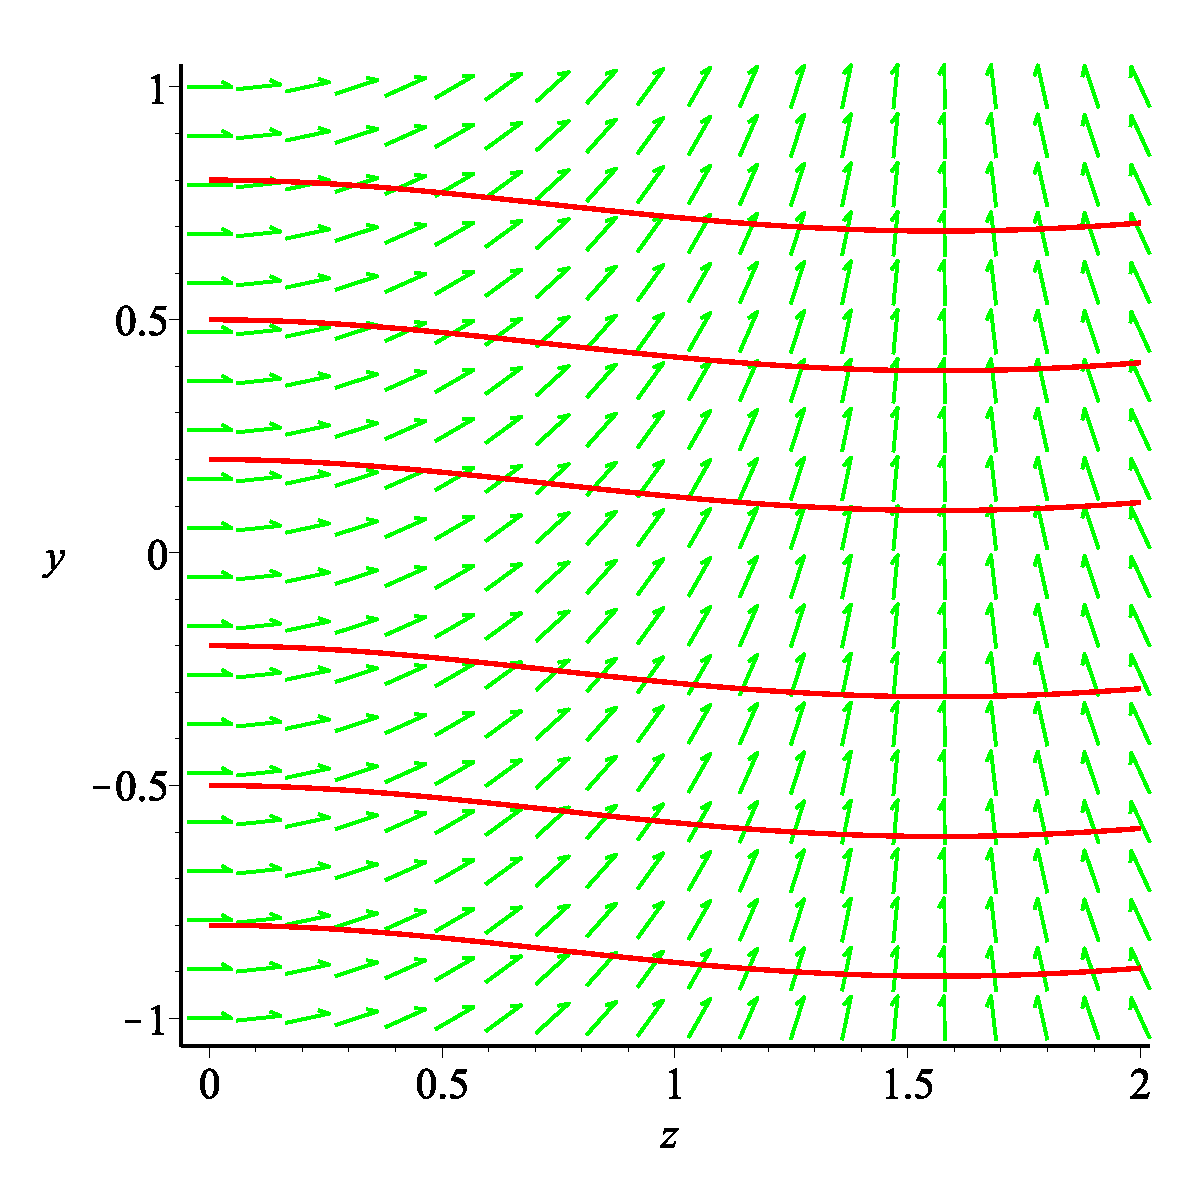
\includegraphics[scale=0.2]{Visualization2}
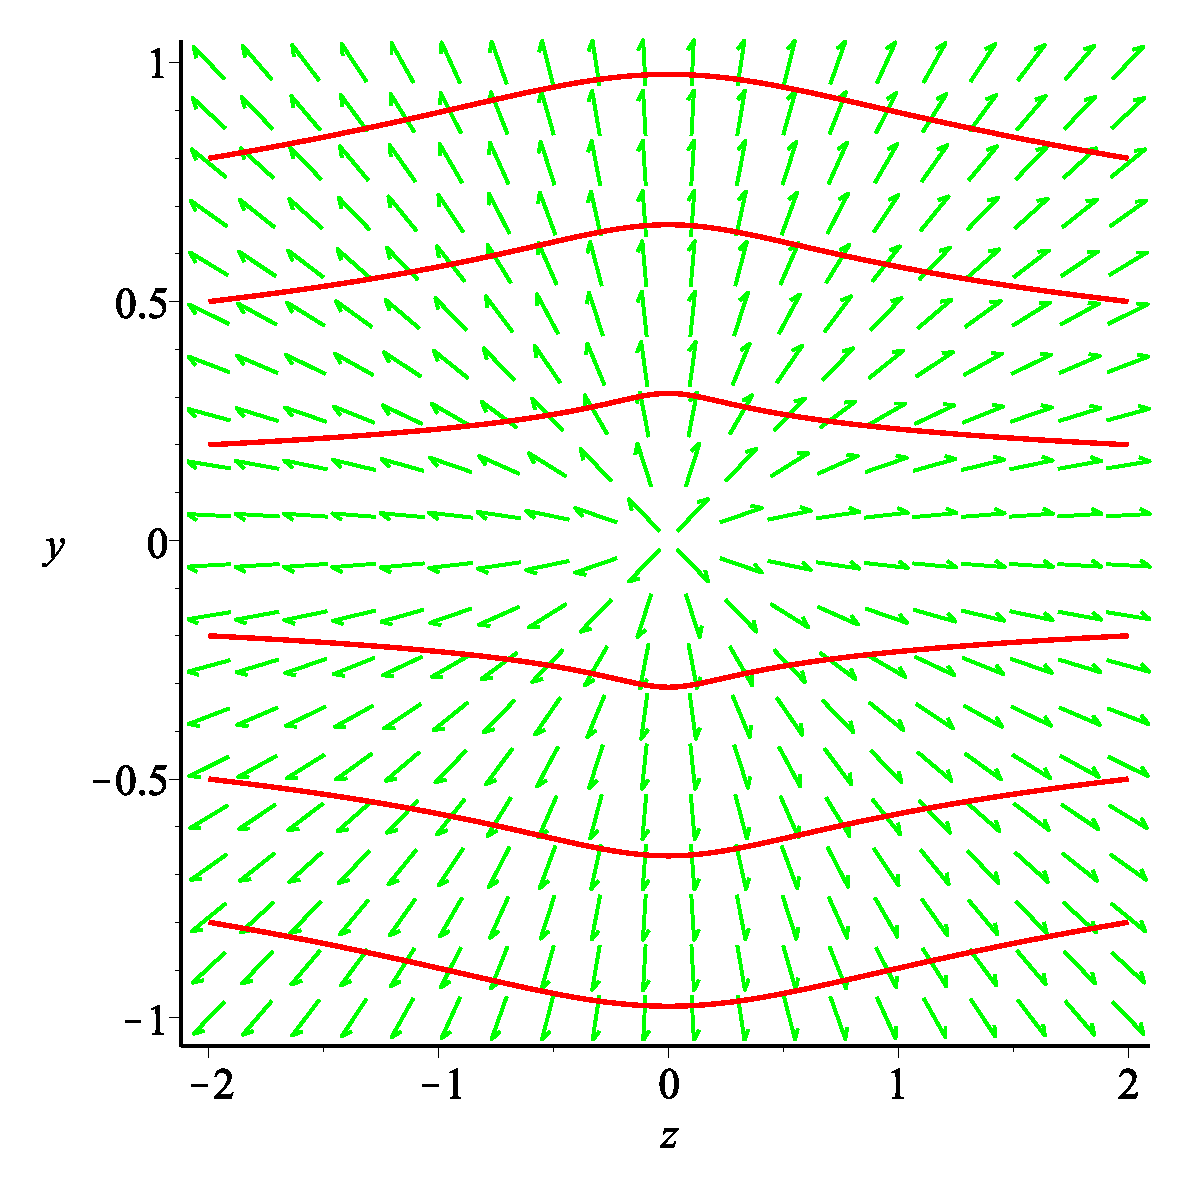
\includegraphics[scale=0.2]{Visualization1}
\caption{Ray tracing in anisotropic media with variable optical axes, $\theta=z$ (left) and $\tan{\theta}=y/z$ (right),  the  green arrows  indicate orientations of the third principle axis and the red lines  indicate ray trajectories  in the media.}
\label{curvedspace2}
\end{figure}




It has been shown in the Fig. \ref{curvedspace2},  that the light geodesics through these media
 are not straight lines. Also, it seems that these surfaces are under tensions.  Therefore,  we expect non-zero Riemann tensor for them. For better investigation of the effective geometry of these media, in the following,  we obtain the metric and Riemann curvature tensor of these surfaces. 
 
The metric of  these two dimensional distorted surfaces, Fig \ref{curvedspace2}, can be constructed by choosing two bases as 
\begin{eqnarray}\label{base}
e_{1}=c_{1}
\begin{pmatrix}
1\\0
\end{pmatrix} \qquad
e_{2}=c_{2}
\begin{pmatrix}
0\\1
\end{pmatrix}
\end{eqnarray}

 where coefficients $c_{1}$ and $c_{2}$  are scalar functions provide null geodesics condition, $\mathrm{d}s^{2}=0$. Using these bases(\ref{base}), we obtain the metric components \cite{leonhardt2012geometry}:
 
\begin{eqnarray}
&g_{ij}=e_{i}\cdot e_{j}.
\end{eqnarray}

Therefore, the space-time metric for the extraordinary light is,  

\begin{align}\label{m2}
\begin{split}
&\mathbf{g}(2+1) =\\
&\begin{pmatrix}
-1&0&0\\
\\ 0& \dfrac{\varepsilon_{2}\varepsilon_{3}\left({\varepsilon_{2} \sin^{2}{\theta} + \varepsilon_{3}\cos^{2}}\right)}{\left({\varepsilon_{2}^{2} \sin^{2}{\theta} + \varepsilon_{3}^{2}\cos^{2}}\right)}&0\\
0&0&\dfrac{\varepsilon_{2}\varepsilon_{3}\left({\varepsilon_{2} \sin^{2}{\theta} + \varepsilon_{3}\cos^{2}}\right)}{\left({\varepsilon_{2}^{2} \sin^{2}{\theta} + \varepsilon_{3}^{2}\cos^{2}}\right)}
\end{pmatrix}.
\end{split}
\end{align}

Which resemble  the metric (\ref{r1.element}), for the extraordinary ray.
 
On the other hand, Riemann curvature tensor given by \cite{leonhardt2012geometry}
\begin{equation}\label{Riemann}
R^{i}_{jkl}\equiv \Gamma^{i}_{jl,k}-\Gamma^{i}_{jk,l}+\Gamma^{i}_{mk}\Gamma^{m}_{jl}-\Gamma^{i}_{ml}\Gamma^{m}_{jk}
\end{equation}

where $\Gamma^{i}_{jk}$ is Christoffel symbol and the comma notation "$,$" refers to partial differentiation.  The Christoffel symbol can be expressed in terms of the metric component as
\begin{equation}\label{cr}
\Gamma^{i}_{jk}=\dfrac{1}{2} g^{il}(g_{lj,k}+g_{lk,j}-g_{jk,l})
\end{equation}

For the metric (\ref{m2}), which is conformally two dimensional flat spaces, $g_{ij}=n^{2}\delta_{ij}$, we can obtain Christoffel symbol as

\begin{equation}\label{cr1}
\Gamma^{i}_{ij}=\dfrac{1}{2n^{2}}n^{2}_{,j}
\end{equation}
Using relation (\ref{cr1}), Riemann curvature tensor, (\ref{Riemann}) can be achieved as 
\begin{equation}
\begin{split}
&R_{11}=R_{22}=\\
&\dfrac{1}{2n^{4}} \lbrace (\dfrac{\partial}{\partial z}n^{2})^{2} +(\dfrac{\partial}{\partial y}n^{2})^{2}\rbrace -\dfrac{1}{2n^{2}}\lbrace(\dfrac{\partial}{\partial z}\dfrac{\partial}{\partial z}n^{2})+(\dfrac{\partial}{\partial y}\dfrac{\partial}{\partial y}n^{2})\rbrace
\end{split}
\end{equation}
We calculate this tensor for the two above example of the variable axes media, $\tan{\theta}=y/z$ and $\theta=z$ and find that 
 \begin{equation}
R_{ii}\neq 0.
\end{equation}

Consequently, the medium with $\tan{\theta}=y/z$ and $\theta=z$ have a non-zero Riemann curvature tensor and appears as a curved space for the extraordinary light. Therefore, we can use variable optical axes media for realizing curved space time in the laboratory. According to the left side of Fig. \ref{curvedspace2}, space has stretched in such a way that extraordinary light modes can not pass through the centre of the plane. Consequently, If one puts an object in this area, the object is hidden. Hence, we can also use these media for cloaking devices.

 
\section{Conclusion}\label{conclusion}

In this paper, we have studied the effective geometry of the impedance-matched and non-impedance-matched anisotropic media for normal incident light.  We obtain the effective geometry by calculating the optical lines element for each kind, based on eigenvalue equation method. In the impedance-matched media, light rays do not split; there is a single direction of propagation for each angle of incidence. This direction coincides with the extraordinary ray's direction in the electric media. In our paper, the metric for the light in the impedance-matched media is obtained, which is the same as one might get from transformation optics method. 
In the non-impedance-matched media, for the ordinary and the extraordinary modes in birefringent medium, we associate two general space-time metrics. For the extraordinary mode, we have shown the metric depends on the principle values of the permittivity tensor as well as the orientation of the optical axes. A comparison between the two metrics, one from the impedance-matched medium and the other, from the extraordinary mode in electric medium, shows that they are equivalent. As an example of realization of curved space-time in a non-impedance-matched medium, we obtained the Rindler space-time, by adopting a specific value of $\varepsilon_{1}$ for the ordinary mode.  
In the end, we introduce the family of media with variable optical axes and indicate the role of the directional variability of the optical axes in forming the effective metric. We show if the optical axes orientation varies, would results in the emergence of effective geometry in the medium. Our finding is a new method for manipulation of electromagnetic waves.  
 

\section*{Acknowledgment}
S.A.M, R.R wish to thank the office of graduate studies of the university of Isfahan for their support.

\bibliography{mybib}

\end{document}
